
\documentclass[aspectratio=169]{beamer}

\usetheme{Rochester}
\usepackage{tikz}
\usepackage{circuitikz}
\usepackage{xcolor}
\usepackage{ifthen}
\usepackage{nicematrix}
\ctikzset{logic ports=european}
\ctikzset{tripoles/european not symbol=ieee circle}
\usetikzlibrary {positioning}
\usetikzlibrary{overlay-beamer-styles, calc}

\title{Halbaddierer, Volladdierer, Ripple-Carry-Addierer} 
\author{Michel Bode}
\date{11.06.2024}

\begin{document}

\tikzset{
	every node/.style={inner sep=0.5mm}
}
\tikzset{
  greenOn/.style={alt=#1{draw, rectangle, green!70!black}{}}}
\tikzset{
  blueOn/.style={alt=#1{draw, rectangle, blue}{}}}
\tikzset{
  drawRedOn/.style={alt=#1{red, thick}{}}}
	
	\begin{frame}
		\titlepage 
	\end{frame}
	
	\begin{frame}{Einordnung}

		\begin{block}{Übergeordnetes Ziel}
			Berechnung beliebig komplexer Funktionen 
		\end{block}
		
		Als bekannt vorausgesetzt:
		\begin{itemize}
			\item Logische Ausdrücke
			\item Logikgatter und deren Darstellung
			\item Wahrheitstabellen
		\end{itemize}

		In dieser Vorlesung:
		\begin{itemize}
			\item Addition einzelner Bits
			\item Kombination dieser zur Addition von Ganzzahlen (Int)
		\end{itemize}

		Ausblick:
		\begin{itemize}
			\item Bit/Int-Addition ist Grundlage so gut wie aller mathematischen Berechnungen (ALU, FPU, Steuerwerk, \dots)
		\end{itemize}
		
	\end{frame}

	\begin{frame}{Motivation}

		\begin{block}{Schätzfrage}
			Wie viele Bit-Additionen werden für die Berechnung der Quadratwurzel einer Gleitkommazahl einfacher Genauigkeit (32 bit float) benötigt?

			\uncover<2->
			{
				\begin{center}
					Typischerweise mehr als 4000!
				\end{center} 	
			}
		\end{block}
		
	\end{frame}

	\begin{frame}{Addition von Binärzahlen\only<3-5>{ -- Halbaddierer}\only<6-8>{ -- Volladdierer}\only<9->{ -- Ripple-Carry-Addierer}}
		\begin{minipage}[c][2.4cm][c]{\linewidth}
			
		\visible<2->{
		\begin{center}
		\begin{tikzpicture}
			
			\node[] (a) {\color{black}1};
			\node[] (b) [right=0.2 of a] {\color{black}1};
			\node[] (c) [right=0.2 of b] {\color{black}0};
			\node[] (d) [right=0.2 of c] {\color{black}1};
			\node[] (e) [right=0.2 of d] {\color{black}0};
			\node[] (f) [right=0.2 of e] {\color{black}0};
			\node[greenOn=<6-8>] (g) [right=0.2 of f] {\color{black}1};
			\node[greenOn=<3-5>] (h) [right=0.2 of g] {\color{black}0};
			\node[] (aa) [below=0.1 of a] {\color{black}0};
			\node[] (bb) [below=0.1 of b] {\color{black}1};
			\node[] (cc) [below=0.1 of c] {\color{black}1};
			\node[] (dd) [below=0.1 of d] {\color{black}1};
			\node[] (ee) [below=0.1 of e] {\color{black}0};
			\node[] (ff) [below=0.1 of f] {\color{black}1};
			\node[greenOn=<6-8>] (gg) [below=0.1 of g] {\color{black}1};
			\node[greenOn=<3-5>] (hh) [below=0.1 of h] {\color{black}1};
			\node[] (plus) [left=0.5 of aa] {\color{black}+};
			\coordinate[below=0.2 of plus.south west]  (pline);
			\coordinate[below=0.2 of hh.south east]  (hline);
			\path[draw, thin] (pline) -- (hline);
			\node[] (sa) [below=0.3 of aa] {\color{black}0};
			\node[] (sb) [below=0.3 of bb] {\color{black}1};
			\node[] (sc) [below=0.3 of cc] {\color{black}0};
			\node[] (sd) [below=0.3 of dd] {\color{black}0};
			\node[] (se) [below=0.3 of ee] {\color{black}1};
			\node[] (sf) [below=0.3 of ff] {\color{black}0};
			\node[blueOn=<6-8>] (sg) [below=0.3 of gg] {\color{black}0};
			\node[blueOn=<3-5>] (sh) [below=0.3 of hh] {\color{black}1};
			\node[] (pa) [left=0.1 of sa] {\color{black}1};
			\node[below left= 2mm and 2mm of aa.north] (caa) {\color{black}\tiny 1};
			\node[below left= 2mm and 2mm of bb.north] (cbb) {\color{black}\tiny 1};
			\node[below left= 2mm and 2mm of cc.north] (ccc) {\color{black}\tiny 1};
			\node[below left= 2mm and 2mm of dd.north] (cdd) {\color{black}\tiny 1};
			\node[below left= 2mm and 2mm of ee.north] (cee) {\color{black}\tiny 0};
			\node[below left= 2mm and 2mm of ff.north] (cff) {\color{black}\tiny 1};
			\node[below left= 2mm and 2mm of gg.north, blueOn=<6-8>] (cgg) {\color{black}\tiny 1};
			\node[below left= 2mm and 2mm of hh.north, blueOn=<3-5>, greenOn=<6-8>] (chh) {\color{black}\tiny 0};
		\end{tikzpicture}
		\end{center}}
		\end{minipage}
		\vspace{0.0cm}

		\begin{minipage}[t][4cm][t]{\linewidth}
			\only<3-8>{
				\begin{columns}[T]
					\begin{column}{.48\textwidth}
					\only<1-5>{
						Als Binärziffern:
						\[{\color{green!70!black}a} + {\color{green!70!black}b} =  {\color{blue}\overline{cs}}{\color{white}\overline{c_{o}}}\]
						\visible<4-5>{Als logischer Ausdruck:
						\begin{align*} 
							{\color{blue}s} &=  {\color{green!70!black}a} \oplus {\color{green!70!black}b}\\ 
							{\color{blue}c} &=  {\color{green!70!black}a} \wedge {\color{green!70!black}b}
						\end{align*}}
					}\only<6-8>{
						Als Binärziffern:
						\[{\color{green!70!black}a} + {\color{green!70!black}b} + {\color{green!70!black}c_{in}} =  {\color{blue}\overline{c_{out}s}}\]
						\visible<7-8>{Als logischer Ausdruck:
						\begin{align*} 
							{\color{blue}s} &=  {\color{green!70!black}a} \oplus {\color{green!70!black}b} \oplus {\color{green!70!black}c_{in}}\\ 
							{\color{blue}c_{out}} &=  ({\color{green!70!black}a} \wedge {\color{green!70!black}b}) \vee (({\color{green!70!black}a} \oplus {\color{green!70!black}b}) \wedge {\color{green!70!black}c_{in}})
						\end{align*}}
					}
					\vfill
					\end{column}
					\hfill
					\begin{column}{.48\textwidth}
						\only<2-4>{
							Wahrheitstabelle:\\
							\vspace{0.3cm}
							\hspace*{0.5cm}$\begin{array}{ |cc|cc| } 
								\hline
								{\color{green!70!black}a} & {\color{green!70!black}b} & {\color{blue}c} & {\color{blue}s} \\
								\hline
								0 & 0 & \tikz[overlay,remember picture]{\node [] (c1) {}}0 & \tikz[overlay,remember picture]{\node [] (s1) {}}0 \\ 
								0 & 1 & 0 & 1 \\ 
								1 & 0 & 0 & 1 \\ 
								1 & 1 & \tikz[overlay,remember picture]{\node [] (c2) {}}1 & \tikz[overlay,remember picture]{\node [] (s2) {}}0 \\ 
								\hline
							\end{array}$
						}\only<5>{
							Schaltbild:\\
							\vspace{0.3cm}
							\begin{circuitikz}[]
								\draw (0,0) node[xor port](xor){};
								\draw (xor.in 1) -- ++(-0.7,0) node[left=0.1](a){$a$}
								(xor.in 2) -- ++(-0.7,0) node[left=0.1](b){$b$}
								(xor.out) -- ++(0.4,0) node[right=0.1](s){$s$};
								\node[draw, and port,below=0.2 of xor](and){};
								\draw (and.in 1) -- (and.in 1 |- a)  node[circ] {}
								(and.in 2) -- ++(-0.3,0) node[](t){} -- (t |- b)  node[circ] {}
								(and.out) -- ++(0.4,0) node[right=0.1](c){$c$};
							\end{circuitikz}
						}\only<6-7>{
							Wahrheitstabelle:\\
							\vspace{0.2cm}
							\hspace*{0.5cm}\resizebox{!}{1.78cm}{$\begin{array}{ |ccc|cc| } 
								\hline
								{\color{green!70!black}a} & {\color{green!70!black}b} & {\color{green!70!black}c_{in}} & {\color{blue}c_{out}} & {\color{blue}s} \\
								\hline
								0 & 0 & 0 & \tikz[overlay,remember picture]{\node [] (c3) {}}0 & \tikz[overlay,remember picture]{\node [] (s3) {}}0 \\ 
								0 & 0 & 1 & 0 & 1 \\ 
								0 & 1 & 0 & 0 & 1 \\ 
								0 & 1 & 1 & 1 & 0 \\ 
								1 & 0 & 0 & 0 & 1 \\ 
								1 & 0 & 1 & 1 & 0 \\ 
								1 & 1 & 0 & 1 & 0 \\ 
								1 & 1 & 1 & \tikz[overlay,remember picture]{\node [] (c4) {}}1 & \tikz[overlay,remember picture]{\node [] (s4) {}}1 \\ 
								\hline
							\end{array}$}
						}\only<8>{
							Schaltbild:\\
							\vspace{0.3cm}
							\resizebox{.9\textwidth}{!}{
							\begin{circuitikz}[]
								\draw (0,0) node[xor port](xor1){};
								\draw (xor1.in 1) -- ++(-0.7,0) node[](leftCircle){} node[left=0.1](a){$a$}
								(xor1.in 2) -- ++(-0.7,0) node[left=0.1](b){$b$};
								\node[draw, and port,below=0.2 of xor](and1){};
								\draw (and1.in 1) -- (and1.in 1 |- a)  node[circ]{}
								(and1.in 2) -- ++(-0.3,0) node[](t){} -- (t |- b)  node[circ] {};
								\draw (xor1.out) node[](t4){} -- ++(0.5,0) node[xor port, anchor=in 1](xor2){};
								\node[draw, and port,below=0.5 of xor2](and2){};
								\draw (and2.in 2) node[](t2){} -- (t2 -| leftCircle) node[left=0.1](c){$c_{in}$};
								\draw (and2.in 1) -- ++(-0.15,0)  node[](t5){} |- (t5 |- t4) node[circ](){};
								\draw (xor2.in 2) -| (and2.in 2) node[circ](){};
								\draw (and2.out) -| ++(0,-0.3) node[or port, anchor=in 1](or){};
								\draw (or.in 2) -| (and1.out);
								\draw (or.out) node[](rightCircle){} node[right=0.1](cout){$c_{out}$};
								\draw (xor2.out) node[](t3){} -- (t3 -| rightCircle) node[right=0.1](s){$s$};
								\draw[red,dotted]     ($(xor1.north west)+(-.5,.55)$) rectangle ($(and1.south east)+(-.2,-.15)$);
								\draw[red,dotted]     ($(xor2.north west)+(-.35,.55)$) rectangle ($(and2.south east)+(-.2,-.15)$);
								\draw ($(xor2.north west)+(0,.35)$) node[](){HA}
								($(xor1.north west)+(-.15,.35)$) node[](){HA};
							\end{circuitikz}}
						}
					\end{column}
				\end{columns}
			}\only<9>{
				\vspace{0.4cm}
				Schaltbild:
				\begin{center}
				\resizebox{.9\textwidth}{!}{
				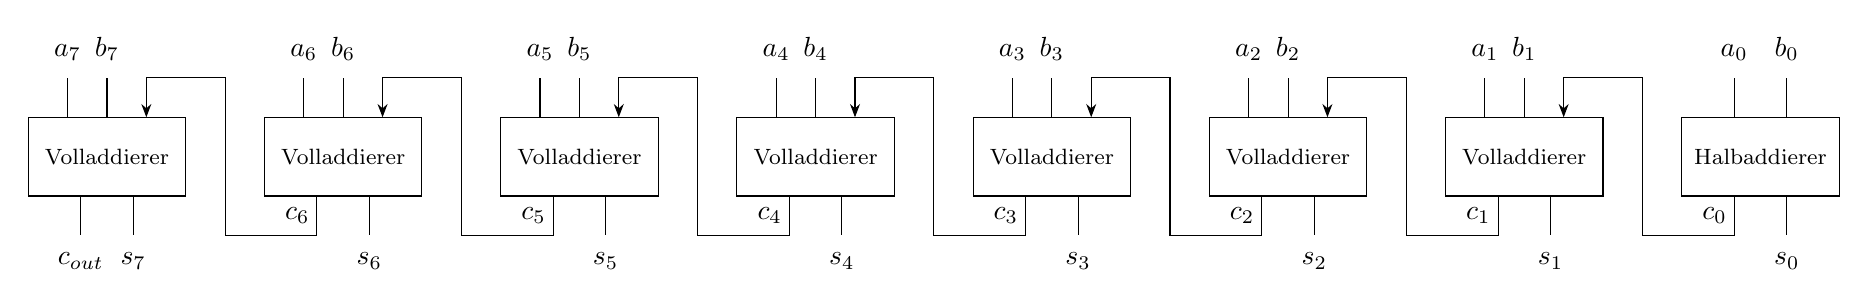
\begin{tikzpicture}
					\foreach \x in {0,3,...,21}
					{
						\pgfmathtruncatemacro{\num}{7 - \x/3}
						\draw (\x,0) rectangle +(2,-1)
						\ifnum\num>0
							(\x,0) +(1,-0.5) node[](){\footnotesize Volladdierer};
							\draw[{Stealth}-](\x,0) ++(1.5,0)  |- ++(1,0.5) |- ++(1.16666,-2) -- ++(0,0.5);
							\draw (\x+0.5,0) -- ++(0,0.5) node[](){} node[above=0.1](){$a_{\num}$};
							\draw (\x+1,0) -- ++(0,0.5) node[](){} node[above=0.1](){$b_{\num}$};
						\else
							(\x,0) +(1,-0.5) node[](){\footnotesize Halbaddierer};
							\draw (\x+0.666667,0) -- ++(0,0.5) node[](){} node[above=0.1](){$a_{\num}$};
							\draw (\x+1.333333,0) -- ++(0,0.5) node[](){} node[above=0.1](){$b_{\num}$};
						\fi
						\draw (\x+1.333333,-1) -- ++(0,-0.5) node[](){} node[below=0.1](){$s_{\num}$};
						\ifnum\num<7 
							\draw (\x+0.666667,-1.5) ++ (-0.25,0.25) node[](){$c_{\num}$};
						\else
							\draw (\x+0.666667,-1) -- ++(0,-0.5) node[](){} node[below=0.1](){$c_{out}$};
						\fi 
					}
				\end{tikzpicture}
				}
				\end{center}
			}
		\end{minipage}
	\end{frame}

	\begin{frame}{Ripple-Carry-Addierer - der kritische Pfad}
		Berechnung von $11011011 + 00100101$, iterativ in diskreten Zeitschritten:
		
		\begin{center}
			\resizebox{.9\textwidth}{!}{
			\begin{tikzpicture}
				% fix wriggle
				\draw (1.333333,-1) ++(0,-0.5) node[white](){} node[below=0.1](){$\mathcolor{white}{\mathbf{0}}$};
				
				\foreach \x in {0,3,...,21}
				{
					\pgfmathtruncatemacro{\num}{7 - \x/3}
					\pgfmathtruncatemacro{\zeroMax}{\num + 1}
					\pgfmathtruncatemacro{\oneMin}{\num + 2}
					\pgfmathtruncatemacro{\oneMinPlusOne}{\num + 3}
					\draw (\x,0) rectangle +(2,-1)
					\ifnum\num>0
						(\x,0) +(1,-0.5) node[](){\footnotesize Volladdierer};
						\draw[{Stealth}-,drawRedOn=<\zeroMax>](\x,0) ++(1.5,0)  |- ++(1,0.5) |- ++(1.16666,-2) -- ++(0,0.5);
						\draw (\x+0.5,0) -- ++(0,0.5) node[](){};
						\draw (\x+1,0) -- ++(0,0.5) node[](){};
						\draw (\x+1.333333,-1) -- ++(0,-0.5) node[](){} node[below=0.1](){\only<1>{$0$}\only<2-\zeroMax>{$1$}\only<\oneMin>{$\mathcolor{green!70!black}{\mathbf{0}}$}\only<\oneMinPlusOne->{$0$}};
					\else
						(\x,0) +(1,-0.5) node[](){\footnotesize Halbaddierer};
						\draw (\x+0.666667,0) -- ++(0,0.5) node[](){};
						\draw (\x+1.333333,0) -- ++(0,0.5) node[](){};
						\draw (\x+1.333333,-1) -- ++(0,-0.5) node[](){} node[below=0.1](){\only<1>{$0$}\only<2>{$\mathcolor{green!70!black}{\mathbf{0}}$}\only<3->{$0$}};
					\fi
					\ifnum\num<7 
						\draw (\x+0.666667,-1.5) ++ (-0.25,0.25) node[](){\only<1-\zeroMax>{$0$}\only<\oneMin>{$\mathcolor{green!70!black}{\mathbf{1}}$}\only<\oneMinPlusOne->{$1$}};
					\else
						\draw (\x+0.666667,-1) -- ++(0,-0.5) node[](){} node[below=0.1](){\only<1-8>{$0$}\only<9>{$\mathcolor{green!70!black}{\mathbf{1}}$}\only<10->{$1$}};
					\fi 
					\only<\zeroMax>{\draw (0,-0.5) node[left=0.5, anchor=east](){$t=\num$};}
				}
				\draw (0.5,0.8) node[](){$1$} ++(3,0) node[](){$1$} ++(3,0) node[](){$0$} ++(3,0) node[](){$1$}
				        ++(3,0) node[](){$1$} ++(3,0) node[](){$0$} ++(3,0) node[](){$1$} ++(3.166666666,0) node[](){$1$};
				\draw   (1,0.8) node[](){$0$} ++(3,0) node[](){$0$} ++(3,0) node[](){$1$} ++(3,0) node[](){$0$}
						++(3,0) node[](){$0$} ++(3,0) node[](){$1$} ++(3,0) node[](){$0$} ++(3.33333333,0) node[](){$1$};
				\only<9->{\draw (0,-0.5) node[left=0.5, anchor=east](){$t=8$};}
			\end{tikzpicture}
			}
		\end{center}
		\visible<10->{
			\begin{itemize}
				\item Zeit der Propagierung des Carry-Bits ist kritisch
				\item Gesamtlaufzeit skaliert linear mit Anzahl Bits
				\visible<11->{\item schnellere Addierwerke möglich, kosten aber mehr (Platz, Strom, Bauteile)}
			\end{itemize}
		}
	\end{frame}

	\begin{frame}{Aufbau des Volladdierers}
		\begin{center}
			\resizebox{!}{2.5cm}{
			\begin{circuitikz}[]
				\colorlet{highlight}{orange}
				\draw (0,0) node[xor port](xor1){};
				\draw (xor1.in 1) -- ++(-0.7,0) node[](leftCircle){} node[left=0.1](a){$a$}
				(xor1.in 2) -- ++(-0.7,0) node[](){} node[left=0.1](b){$b$};
				\node[draw, and port,below=0.2 of xor1](and1){};
				\draw (and1.in 1) -- (and1.in 1 |- a)  node[circ]{}
				(and1.in 2) -- ++(-0.3,0) node[](t){} -- (t |- b)  node[circ] {};
				\draw (xor1.out) node[](t4){} -- ++(0.5,0) node[xor port, anchor=in 1](xor2){};
				\node[draw, and port,below=0.5 of xor2, fill=highlight](and2){};
				\draw[highlight, thick] (and2.in 2) node[](t2){} -- (t2 -| leftCircle) node[](cCirc){} node[left=0.1, thick, highlight](c){$c_{in}$};
				\draw (and2.in 1) -- ++(-0.15,0)  node[](t5){} |- (t5 |- t4) node[circ](){};
				\draw (xor2.in 2) -| (and2.in 2);
				\draw (and2.out) -| ++(0,-0.3) node[or port, anchor=in 1, fill=highlight](or){};
				\draw (or.in 2) -| (and1.out);
				\draw (or.out) node[](rightCircle){} node[right=0.1, thick, highlight](cout){$c_{out}$};
				\draw (xor2.out) node[](t3){} -- (t3 -| rightCircle) node[](){} node[right=0.1](s){$s$};
				\draw[highlight, thick] (t2) -- (and2.bin 2) (and2.bout) --  (and2.out) |- (or.bin 1) (or.bout) -- (or.out);
				\draw[thick] (and2.bin 2) ++(0,0.1) -- ++(0,-0.2) (and2.bout) ++(0,0.1) -- ++(0,-0.2)
				             (or.bin 1) ++(0,0.1) -- ++(0,-0.2) (or.bout) ++(0,0.1) -- ++(0,-0.2)  ;
				\draw (and2.in 2) node[circ](){};
				\draw[red,dotted]     ($(xor1.north west)+(-.5,.55)$) rectangle ($(and1.south east)+(-.2,-.15)$);
				\draw[red,dotted]     ($(xor2.north west)+(-.35,.55)$) rectangle ($(and2.south east)+(-.2,-.15)$);
				\draw ($(xor2.north west)+(0,.35)$) node[](){HA}
				($(xor1.north west)+(-.15,.35)$) node[](){HA};
			\end{circuitikz}}
		\end{center}
		\visible<2->{
		\begin{columns}
			\begin{column}[T]{0.58\textwidth}
				\begin{itemize}
					\item $c_{out}$ hängt von $c_{in}$ und $a+b$ ab
					\item $c_{out}$ aus $c_{in}$ und $a+b$ nicht mit nur einem einfachen Logikgatter darstellbar
					\item als integrierter Schaltkreis sind Abkürzungen möglich
				\end{itemize}
			\end{column}
			\begin{column}[T]{0.38\textwidth}
				$\begin{NiceArray}{cc|cc|}[]
					\Block{2-2}{} & & \Block{1-2}{c_{in}}\\
					 & & 0 & 1  \\
					\hline
					\Block{3-1}{\rotatebox{90}{a+b}}
					& 0 & 0 & 0\\
					& 1 & 0 & 1\\
					& 2 & 1 & 1\\
				\end{NiceArray}$
			\end{column}
		\end{columns}}
	\end{frame}

	\begin{frame}{Alternative Schaltbilder}
		\begin{columns}
			\begin{column}[T]{.48\textwidth}
				\begin{minipage}[t][3.0cm][t]{\linewidth}
				\resizebox{.9\textwidth}{!}{
				\begin{circuitikz}[]
					\draw (0,0) node[xor port](xor1){};
					\draw (xor1.in 1) -- ++(-0.7,0) node[](leftCircle){} node[left=0.1](a){$a$}
					(xor1.in 2) -- ++(-0.7,0) node[](){} node[left=0.1](b){$b$};
					\node[draw, and port,below=0.2 of xor1](and1){};
					\draw (and1.in 1) -- (and1.in 1 |- a)  node[circ]{}
					(and1.in 2) -- ++(-0.3,0) node[](t){} -- (t |- b)  node[circ] {};
					\draw (xor1.out) node[](t4){} -- ++(0.5,0) node[xor port, anchor=in 1](xor2){};
					\node[draw, and port,below=0.5 of xor2](and2){};
					\draw (and2.in 2) node[](t2){} -- (t2 -| leftCircle) node[](){} node[left=0.1](c){$c_{in}$};
					\draw (and2.in 1) -- ++(-0.15,0)  node[](t5){} |- (t5 |- t4) node[circ](){};
					\draw (xor2.in 2) -| (and2.in 2) node[circ](){};
					\draw (and2.out) -| ++(0,-0.3) node[or port, anchor=in 1](or){};
					\draw (or.in 2) -| (and1.out);
					\draw (or.out) node[](rightCircle){} node[right=0.1](cout){$c_{out}$};
					\draw (xor2.out) node[](t3){} -- (t3 -| rightCircle) node[](){} node[right=0.1](s){$s$};
				\end{circuitikz}}					
			\end{minipage}
			\resizebox{.9\textwidth}{!}{
				\begin{circuitikz}[]
					\ctikzset{tripoles/european nor port/width=1.0}
					\draw (0,0) node[nor port](nor1){};
					\draw (nor1.in 1) -- ++(-0.3,0) node[](leftCircle){} node[left=0.1](a){$a$}
					(nor1.in 2) -- (nor1.in 2 -| leftCircle) node[](){} node[left=0.1](b){$b$};
					\draw (nor1.out) -- ++(0.05,0) node[circ](t1){} -- ++(0,0.5) node[nor port, anchor=in 2](nor2){};
					\draw (t1) -- ++(0,-0.5) node[nor port, anchor=in 1](nor3){};
					\draw (nor2.in 1) -| (nor1.in 1) node[circ](){};
					\draw (nor3.in 2) -| (nor1.in 2) node[circ](){};
					\draw (nor2.out) -- (nor2.out |- nor1.in 1) node[nor port, anchor=in 1](nor4){};
					\draw (nor3.out) -- (nor4.in 2);
					\draw (nor4.out) -- ++(0.05,0) node[nor port, anchor=in 1](nor5){};
					\draw (nor5.out) -- ++(0.05,0) node[circ](t2){} -- ++(0,0.5) node[nor port, anchor=in 2](nor6){};
					\draw (t2) -- ++(0,-0.5) node[nor port, anchor=in 1](nor7){};
					\draw (nor6.in 1) -| (nor5.in 1) node[circ](){};
					\draw (nor7.in 2) -- (nor7.in 2 -| nor5.in 2) node[circ](t4){} -- (nor5.in 2);
					\draw (nor6.out) -- (nor6.out |- nor5.in 1) node[nor port, anchor=in 1](nor8){};
					\draw (nor7.out) -- (nor8.in 2);
					\draw (nor8.out) -- ++(0.1,0) node[](){} node[right=0.1](s){$s$};
					\draw (nor7.in 1) node[circ](){} -- ++(0,-1) node[](t3){} -- (t3 -| nor8.in 1) node[nor port, anchor=in 1](nor9){};
					\draw (nor9.in 2) -| (nor3.in 1) node[circ](){};
					\draw (nor9.out) -- ++(0.1,0) node[](){} node[right=0.1](cout){$c_{out}$};
					\draw (t4) -- ++(0,-0.3) node[](t5){} -- (t5 -| leftCircle) node[](){} node[left=0.1](cin){$c_{in}$};
				\end{circuitikz}}
			\end{column}
			\begin{column}[T]{.48\textwidth}
				\begin{minipage}[t][2.5cm][t]{\linewidth}
				\resizebox{.9\textwidth}{!}{
				\begin{circuitikz}[]
					\draw (0,0) node[and port](and1){};
					\draw (and1.in 1) -- ++(-0.7,0) node[](leftCircle){} node[left=0.1](a){$a$}
					(and1.in 2) -- ++(-0.7,0) node[](){} node[left=0.1](b){$b$};
					\node[draw, or port,below=0.2 of and1](or1){};
					\draw (or1.in 1) -- (or1.in 1 |- a)  node[circ]{}
					(or1.in 2) -- ++(-0.3,0) node[](t){} -- (t |- b)  node[circ] {};
					\draw (or1.out) -- ++(0.3,0) node[or port, anchor=in 1](or2){};
					\node[draw, and port, below=0.3 of or2](and2){};
					\draw (and2.in 2) -- (and2.in 2 -| leftCircle) node[](){} node[left=0.1](c){$c_{in}$};
					\draw (and2.in 1) -- (or2.in 1) node[circ](){};
					\draw (and2.out) node[or port, anchor=in 2](or3){};
					\draw (or3.in 1) -- (or3.in 1 |- and1.out) node[circ](t){} -- (and1.out);
					\draw (t) node[draw, and port, anchor=in 1](and3){};
					\draw (and3.in 2) -| (or1.out |- c) node[circ](){};
					\draw (or2.in 2) -- (or2.in 2 -| or1.out) node[circ](){};
					\draw (or2.out) -- (or2.out -| or3.out) node[and port, anchor=in 1](and4){};
					\draw (and4.in 2) -- (or3.out);
					\node at (and4.bin 2) [ocirc, left, scale =1.5]{};
					\draw (and3.out) -- (and3.out -| and4.out) node[or port, anchor=in 1](or4){};
					\draw (or4.in 2) -- (and4.out);
					\draw (or4.out) node[](t2){} node[right=0.1](s){$s$};
					\draw (or3.out) node[circ](){} --  (or3.out -| t2) node[](){} node[right=0.1](cout){$c_{out}$};
				\end{circuitikz}}					
			\end{minipage}
			\resizebox{!}{3.5cm}{
				\begin{circuitikz}[]
					\ctikzset{tripoles/european not port/height=.5}
					\draw (0,0) node[and port, number inputs=3](and1){};
					\node[draw, and port,below=0.2 of and1, number inputs=3](and2){};
					\node[draw, and port,below=0.2 of and2, number inputs=3](and3){};
					\node[draw, and port,below=0.2 of and3, number inputs=3](and4){};
					\node[draw, and port,below=0.4 of and4](and5){};
					\node[draw, and port,below=0.2 of and5](and6){};
					\node[draw, and port,below=0.2 of and6](and7){};
					\draw (and2.in 3) -- (and3.in 3) node[](notc){};
					\draw (and2.in 2) -- ++(-0.2,0) node[](notb){} |- (and4.in 2);
					\draw (and3.in 1) -- ++(-0.4,0) node[](nota){} |- (and4.in 1);
					\draw (and1.in 3) -- ++(-0.8,0) node[](c){} -- ( c |- and4.in 3) node[circ](){} -- ( c |- and6.in 2) node[circ](){} -- (and6.in 2);
					\draw (c) |- (and7.in 2);
					\draw (and1.in 2) -- ++(-1,0) node[](b){} -- ( b |- and3.in 2) node[circ](){} -- ( b |- and5.in 2) node[circ](){} -- (and5.in 2);
					\draw (b) |- (and7.in 1);
					\draw (and1.in 1) -- ++(-1.2,0) node[](a){} -- (a |- and2.in 1) node[circ](){} -- ( a |- and5.in 1) node[circ](){} -- (and5.in 1);
					\draw (a) |- (and6.in 1);
					\draw (and2.in 1) -- ++(-3.5,0) node[](ina){} node[left=0.2](){$a$};
					\draw (and3.in 2) -- (and3.in 2 -|ina) node[](inb){} node[left=0.2](){$b$};
					\draw (and4.in 3) -- (and4.in 3 -|ina) node[](inc){} node[left=0.2](){$c_{in}$};
					\draw (ina) -- ++(0.2,0) node[circ](t1){} -- ++(0,-0.5) node[not port,anchor=in 1](not1){};
					\draw (inb) -- (inb -| t1) node[circ](){} -- ++(0,-0.5) node[not port,anchor=in 1](not2){};
					\draw (inc) -- (inc -| t1) node[circ](){} -- ++(0,-0.5) node[not port,anchor=in 1](not3){};
					\draw (not1.out) -| (nota) node[circ](){};
					\draw (not2.out) -- (not2.out -| notb) node[circ](){};
					\draw (not3.out) -| (notc) node[circ](){};
					\draw ($(and2.out)!.5!(and3.out)$) ++(2,0) node[or port, number inputs=4](or1){};
					\draw (and6.out) ++(2,0) node[or port, number inputs=3](or2){};
					\draw (and2.out) |- (or1.in 2) (and3.out) |- (or1.in 3)
					      (and1.out) -| (or1.in 1) (and4.out) -| (or1.in 4);
					\draw (and5.out) -| (or2.in 1) (and7.out) -| (or2.in 3) (and6.out) -- (or2.in 2);
					\draw (or1.out) node[](){} node[right=0.1](){$s$};
					\draw (or2.out) node[](){} node[right=0.1](){$c_{out}$};
				\end{circuitikz}}
			\end{column}
		\end{columns}
	\end{frame}
	
	\begin{frame}{Was Sie mitnehmen sollten}
		\begin{block}{}
			Addierer sind die essentiellen Bausteine für die Berechnung mathematischer Funktionen auf dem Computer.
		\end{block}
		\visible<2->{
		\begin{block}{}
			Die Komplexität des Addierens kommt aus der Propagierung des Carry-Bits. 
		\end{block}}
		\visible<3->{
		\begin{block}{}
			Es gibt keine einzelne beste Schaltung für die Addition. Neben Überlegungen zur Relevanz von Latenz und Kosten sind auch zur Verfügung stehende Bauteile zu beachten.
		\end{block}}
	\end{frame}


\end{document}